% Options for packages loaded elsewhere
\PassOptionsToPackage{unicode}{hyperref}
\PassOptionsToPackage{hyphens}{url}
%
\documentclass[
]{article}
\usepackage{amsmath,amssymb}
\usepackage{iftex}
\ifPDFTeX
  \usepackage[T1]{fontenc}
  \usepackage[utf8]{inputenc}
  \usepackage{textcomp} % provide euro and other symbols
\else % if luatex or xetex
  \usepackage{unicode-math} % this also loads fontspec
  \defaultfontfeatures{Scale=MatchLowercase}
  \defaultfontfeatures[\rmfamily]{Ligatures=TeX,Scale=1}
\fi
\usepackage{lmodern}
\ifPDFTeX\else
  % xetex/luatex font selection
\fi
% Use upquote if available, for straight quotes in verbatim environments
\IfFileExists{upquote.sty}{\usepackage{upquote}}{}
\IfFileExists{microtype.sty}{% use microtype if available
  \usepackage[]{microtype}
  \UseMicrotypeSet[protrusion]{basicmath} % disable protrusion for tt fonts
}{}
\makeatletter
\@ifundefined{KOMAClassName}{% if non-KOMA class
  \IfFileExists{parskip.sty}{%
    \usepackage{parskip}
  }{% else
    \setlength{\parindent}{0pt}
    \setlength{\parskip}{6pt plus 2pt minus 1pt}}
}{% if KOMA class
  \KOMAoptions{parskip=half}}
\makeatother
\usepackage{xcolor}
\usepackage[margin=1in]{geometry}
\usepackage{color}
\usepackage{fancyvrb}
\newcommand{\VerbBar}{|}
\newcommand{\VERB}{\Verb[commandchars=\\\{\}]}
\DefineVerbatimEnvironment{Highlighting}{Verbatim}{commandchars=\\\{\}}
% Add ',fontsize=\small' for more characters per line
\usepackage{framed}
\definecolor{shadecolor}{RGB}{248,248,248}
\newenvironment{Shaded}{\begin{snugshade}}{\end{snugshade}}
\newcommand{\AlertTok}[1]{\textcolor[rgb]{0.94,0.16,0.16}{#1}}
\newcommand{\AnnotationTok}[1]{\textcolor[rgb]{0.56,0.35,0.01}{\textbf{\textit{#1}}}}
\newcommand{\AttributeTok}[1]{\textcolor[rgb]{0.13,0.29,0.53}{#1}}
\newcommand{\BaseNTok}[1]{\textcolor[rgb]{0.00,0.00,0.81}{#1}}
\newcommand{\BuiltInTok}[1]{#1}
\newcommand{\CharTok}[1]{\textcolor[rgb]{0.31,0.60,0.02}{#1}}
\newcommand{\CommentTok}[1]{\textcolor[rgb]{0.56,0.35,0.01}{\textit{#1}}}
\newcommand{\CommentVarTok}[1]{\textcolor[rgb]{0.56,0.35,0.01}{\textbf{\textit{#1}}}}
\newcommand{\ConstantTok}[1]{\textcolor[rgb]{0.56,0.35,0.01}{#1}}
\newcommand{\ControlFlowTok}[1]{\textcolor[rgb]{0.13,0.29,0.53}{\textbf{#1}}}
\newcommand{\DataTypeTok}[1]{\textcolor[rgb]{0.13,0.29,0.53}{#1}}
\newcommand{\DecValTok}[1]{\textcolor[rgb]{0.00,0.00,0.81}{#1}}
\newcommand{\DocumentationTok}[1]{\textcolor[rgb]{0.56,0.35,0.01}{\textbf{\textit{#1}}}}
\newcommand{\ErrorTok}[1]{\textcolor[rgb]{0.64,0.00,0.00}{\textbf{#1}}}
\newcommand{\ExtensionTok}[1]{#1}
\newcommand{\FloatTok}[1]{\textcolor[rgb]{0.00,0.00,0.81}{#1}}
\newcommand{\FunctionTok}[1]{\textcolor[rgb]{0.13,0.29,0.53}{\textbf{#1}}}
\newcommand{\ImportTok}[1]{#1}
\newcommand{\InformationTok}[1]{\textcolor[rgb]{0.56,0.35,0.01}{\textbf{\textit{#1}}}}
\newcommand{\KeywordTok}[1]{\textcolor[rgb]{0.13,0.29,0.53}{\textbf{#1}}}
\newcommand{\NormalTok}[1]{#1}
\newcommand{\OperatorTok}[1]{\textcolor[rgb]{0.81,0.36,0.00}{\textbf{#1}}}
\newcommand{\OtherTok}[1]{\textcolor[rgb]{0.56,0.35,0.01}{#1}}
\newcommand{\PreprocessorTok}[1]{\textcolor[rgb]{0.56,0.35,0.01}{\textit{#1}}}
\newcommand{\RegionMarkerTok}[1]{#1}
\newcommand{\SpecialCharTok}[1]{\textcolor[rgb]{0.81,0.36,0.00}{\textbf{#1}}}
\newcommand{\SpecialStringTok}[1]{\textcolor[rgb]{0.31,0.60,0.02}{#1}}
\newcommand{\StringTok}[1]{\textcolor[rgb]{0.31,0.60,0.02}{#1}}
\newcommand{\VariableTok}[1]{\textcolor[rgb]{0.00,0.00,0.00}{#1}}
\newcommand{\VerbatimStringTok}[1]{\textcolor[rgb]{0.31,0.60,0.02}{#1}}
\newcommand{\WarningTok}[1]{\textcolor[rgb]{0.56,0.35,0.01}{\textbf{\textit{#1}}}}
\usepackage{graphicx}
\makeatletter
\def\maxwidth{\ifdim\Gin@nat@width>\linewidth\linewidth\else\Gin@nat@width\fi}
\def\maxheight{\ifdim\Gin@nat@height>\textheight\textheight\else\Gin@nat@height\fi}
\makeatother
% Scale images if necessary, so that they will not overflow the page
% margins by default, and it is still possible to overwrite the defaults
% using explicit options in \includegraphics[width, height, ...]{}
\setkeys{Gin}{width=\maxwidth,height=\maxheight,keepaspectratio}
% Set default figure placement to htbp
\makeatletter
\def\fps@figure{htbp}
\makeatother
\setlength{\emergencystretch}{3em} % prevent overfull lines
\providecommand{\tightlist}{%
  \setlength{\itemsep}{0pt}\setlength{\parskip}{0pt}}
\setcounter{secnumdepth}{-\maxdimen} % remove section numbering
\ifLuaTeX
  \usepackage{selnolig}  % disable illegal ligatures
\fi
\IfFileExists{bookmark.sty}{\usepackage{bookmark}}{\usepackage{hyperref}}
\IfFileExists{xurl.sty}{\usepackage{xurl}}{} % add URL line breaks if available
\urlstyle{same}
\hypersetup{
  pdftitle={Projekt OSP - Spotify Songs},
  pdfauthor={0036539445 Filip Buhinićek, 0036542400 Dominik Zoričić, 0036539188 Nikola Botić},
  hidelinks,
  pdfcreator={LaTeX via pandoc}}

\title{Projekt OSP - Spotify Songs}
\author{0036539445 Filip Buhinićek, 0036542400 Dominik Zoričić,
0036539188 Nikola Botić}
\date{2024-01-25}

\begin{document}
\maketitle

\hypertarget{uvod}{%
\subsection{UVOD}\label{uvod}}

Ovaj skup podataka pruža opsežnu zbirku pjesama s nizom atributa,
uključujući, ali ne ograničavajući se na, popularnost pjesme, žanr,
pojedinosti o izvođaču i niz akustičnih značajki poput tempa, energije
itd. Ovi atributi omogućuju višestruku analizu, od razumijevanja
preferencija slušatelja do istraživanja glazbenih trendova tijekom
vremena.

Naš projekt ima za cilj istražiti ovaj skup podataka kako bismo otkrili
uvide i obrasce u svijetu glazbe na Spotifyju. Za analizu različitih
aspekata podataka koristit ćemo niz statističkih tehnika i metoda
vizualizacije podataka. Projekt je strukturiran za istraživanje skupa
podataka na sveobuhvatan način, počevši od početnog prikupljanja
podataka i predobrade, prelazeći kroz istraživačku analizu podataka.

Krajnji cilj ovog projekta je napraviti analizu podatkovnog skupa, koji
će biti zanimljiv svim čitateljima a ne samo ljubiteljima glazbe.

\hypertarget{opux107enito-o-podatkovnom-skupu}{%
\subsection{OPĆENITO O PODATKOVNOM
SKUPU}\label{opux107enito-o-podatkovnom-skupu}}

Paket spotifyr pruža podatke u sirovom, nefiltriranom obliku, dajući
slobodu i fleksibilnost u oblikovanju analize. Ova neobrađenost znači da
će početni koraci uključivati zadatke pretprocesiranja kao što su
čišćenje nepotrebnih vrijednosti, rukovanje duplikatima i strukturiranje
podataka na način koji najbolje odgovara analitičkim ciljevima.

Neki od zanimljivih atributa podatkovnog skupa kojeg ćemo eksplicitno
prikazivati u našoj obradi su:

\begin{itemize}
\tightlist
\item
  Izvođač (Artist)
\item
  Godina izdanja (Release Year)
\item
  Žanr (Genre)
\item
  Popularnost pjesme (Track Popularity)
\item
  Dužina trajanja (Duration)
\end{itemize}

\hypertarget{uux10ditavanje-podataka-i-procesiranje}{%
\subsection{UČITAVANJE PODATAKA I
PROCESIRANJE}\label{uux10ditavanje-podataka-i-procesiranje}}

\textbf{Učitvanje podataka i odbacivanje nepotrebnih stupaca koji se
neće koristiti u daljnjoj analizi}

Budući da smo odlučili provoditi analizu podataka za koju nam je
potrebno samo određeni skup stupaca, odbacujemo nekorištene stupce tj.
višak informacija.

Na početku, podaci se učitavaju iz CSV datoteke. Ovaj korak je izveden
korištenjem funkcije read\_csv unutar R-a, a zanimljivo je da je
prilikom učitavanja onemogućena automatska detekcija tipova stupaca. Ovo
omogućuje veću kontrolu nad obradom podataka u kasnijim fazama, ali i
veću odgovornost samog programera.

Nakon učitavanja, uslijedila je selekcija određenih stupaca iz skupa
podataka. Ova operacija je ključna jer omogućuje fokusiranje samo na
relevantne i korištene podatke. Stupci koji su zadržani uključuju
identifikacijski broj pjesme, ime pjesme, izvođača, popularnost, datum
izdanja albuma, žanr playliste i trajanje u milisekundama. Takav odabir
stupaca osigurava da su sve bitne informacije zadržane za daljnju
analizu.

Dalje, stupci su preimenovani u nazive koji su intuitivniji i lakši za
razumijevanje. Na primjer, track\_id postaje TrackID, a track\_name
postaje TrackName.

Jedna od bitnih pretvorbi bila je pretvorba trajanja pjesama iz
milisekundi u minute. Ovaj korak je primjer kako podatke možemo
prilagoditi tako da budu u formatu koji je više usklađen s uobičajenim
načinom percipiranja trajanja pjesama.

Stupci Artist i Genre su transformirani u faktore, što je uobičajena
praksa u R-u za rad s kategorijskim podacima. Ovaj korak olakšava
analizu i vizualizaciju podataka koji spadaju u određene kategorije.

Važan dio procesa bila je ekstrakcija godine iz datuma izdanja.
Razvijena je interna funkcija extractYear koja je mogla obraditi
različite formate datuma i izvući relevantnu godinu. Ovo je bilo važno
jer formati datuma nisu bili konzistentni unutar podataka. Na kraju, iz
skupa podataka su uklonjeni svi redovi gdje godina izdanja nije bila
dostupna. Ovo je osiguralo da analiza uključuje samo one zapise gdje su
svi relevantni podaci prisutni.

Kroz ovaj proces, sirovi podaci su transformirani u oblik koji je
pogodniji za detaljnu analizu. Ovaj postupak čišćenja i transformacije
je ključan korak u pripremi podataka, jer osigurava da analiza koja
slijedi bude temeljena na preciznim, relevantnim i dobro strukturiranim
informacijama.

\textbf{Slijedi primjer kako podaci izgledaju nakon uvodne
transformacije:}

\begin{Shaded}
\begin{Highlighting}[]
\FunctionTok{glimpse}\NormalTok{(data)}
\end{Highlighting}
\end{Shaded}

\begin{verbatim}
## Rows: 32,802
## Columns: 7
## $ TrackID     <chr> "6f807x0ima9a1j3VPbc7VN", "0r7CVbZTWZgbTCYdfa2P31", "1z1Hg~
## $ TrackName   <chr> "I Don't Care (with Justin Bieber) - Loud Luxury Remix", "~
## $ Artist      <fct> "Ed Sheeran", "Maroon 5", "Zara Larsson", "The Chainsmoker~
## $ Popularity  <dbl> 66, 67, 70, 60, 69, 67, 62, 69, 68, 67, 58, 67, 67, 68, 63~
## $ ReleaseYear <dbl> 2019, 2019, 2019, 2019, 2019, 2019, 2019, 2019, 2019, 2019~
## $ Genre       <fct> pop, pop, pop, pop, pop, pop, pop, pop, pop, pop, pop, pop~
## $ DurationMin <dbl> 3.25, 2.71, 2.94, 2.82, 3.15, 2.72, 3.13, 3.46, 3.22, 4.22~
\end{verbatim}

\begin{Shaded}
\begin{Highlighting}[]
\FunctionTok{head}\NormalTok{(data)}
\end{Highlighting}
\end{Shaded}

\begin{verbatim}
## # A tibble: 6 x 7
##   TrackID              TrackName Artist Popularity ReleaseYear Genre DurationMin
##   <chr>                <chr>     <fct>       <dbl>       <dbl> <fct>       <dbl>
## 1 6f807x0ima9a1j3VPbc~ I Don't ~ Ed Sh~         66        2019 pop          3.25
## 2 0r7CVbZTWZgbTCYdfa2~ Memories~ Maroo~         67        2019 pop          2.71
## 3 1z1Hg7Vb0AhHDiEmnDE~ All the ~ Zara ~         70        2019 pop          2.94
## 4 75FpbthrwQmzHlBJLuG~ Call You~ The C~         60        2019 pop          2.82
## 5 1e8PAfcKUYoKkxPhrHq~ Someone ~ Lewis~         69        2019 pop          3.15
## 6 7fvUMiyapMsRRxr07cU~ Beautifu~ Ed Sh~         67        2019 pop          2.72
\end{verbatim}

\hypertarget{analiza-procesiranog-podatkovnog-skupa}{%
\subsection{ANALIZA PROCESIRANOG PODATKOVNOG
SKUPA}\label{analiza-procesiranog-podatkovnog-skupa}}

\textbf{\emph{Popularnost žanrova na Spotifyu}}

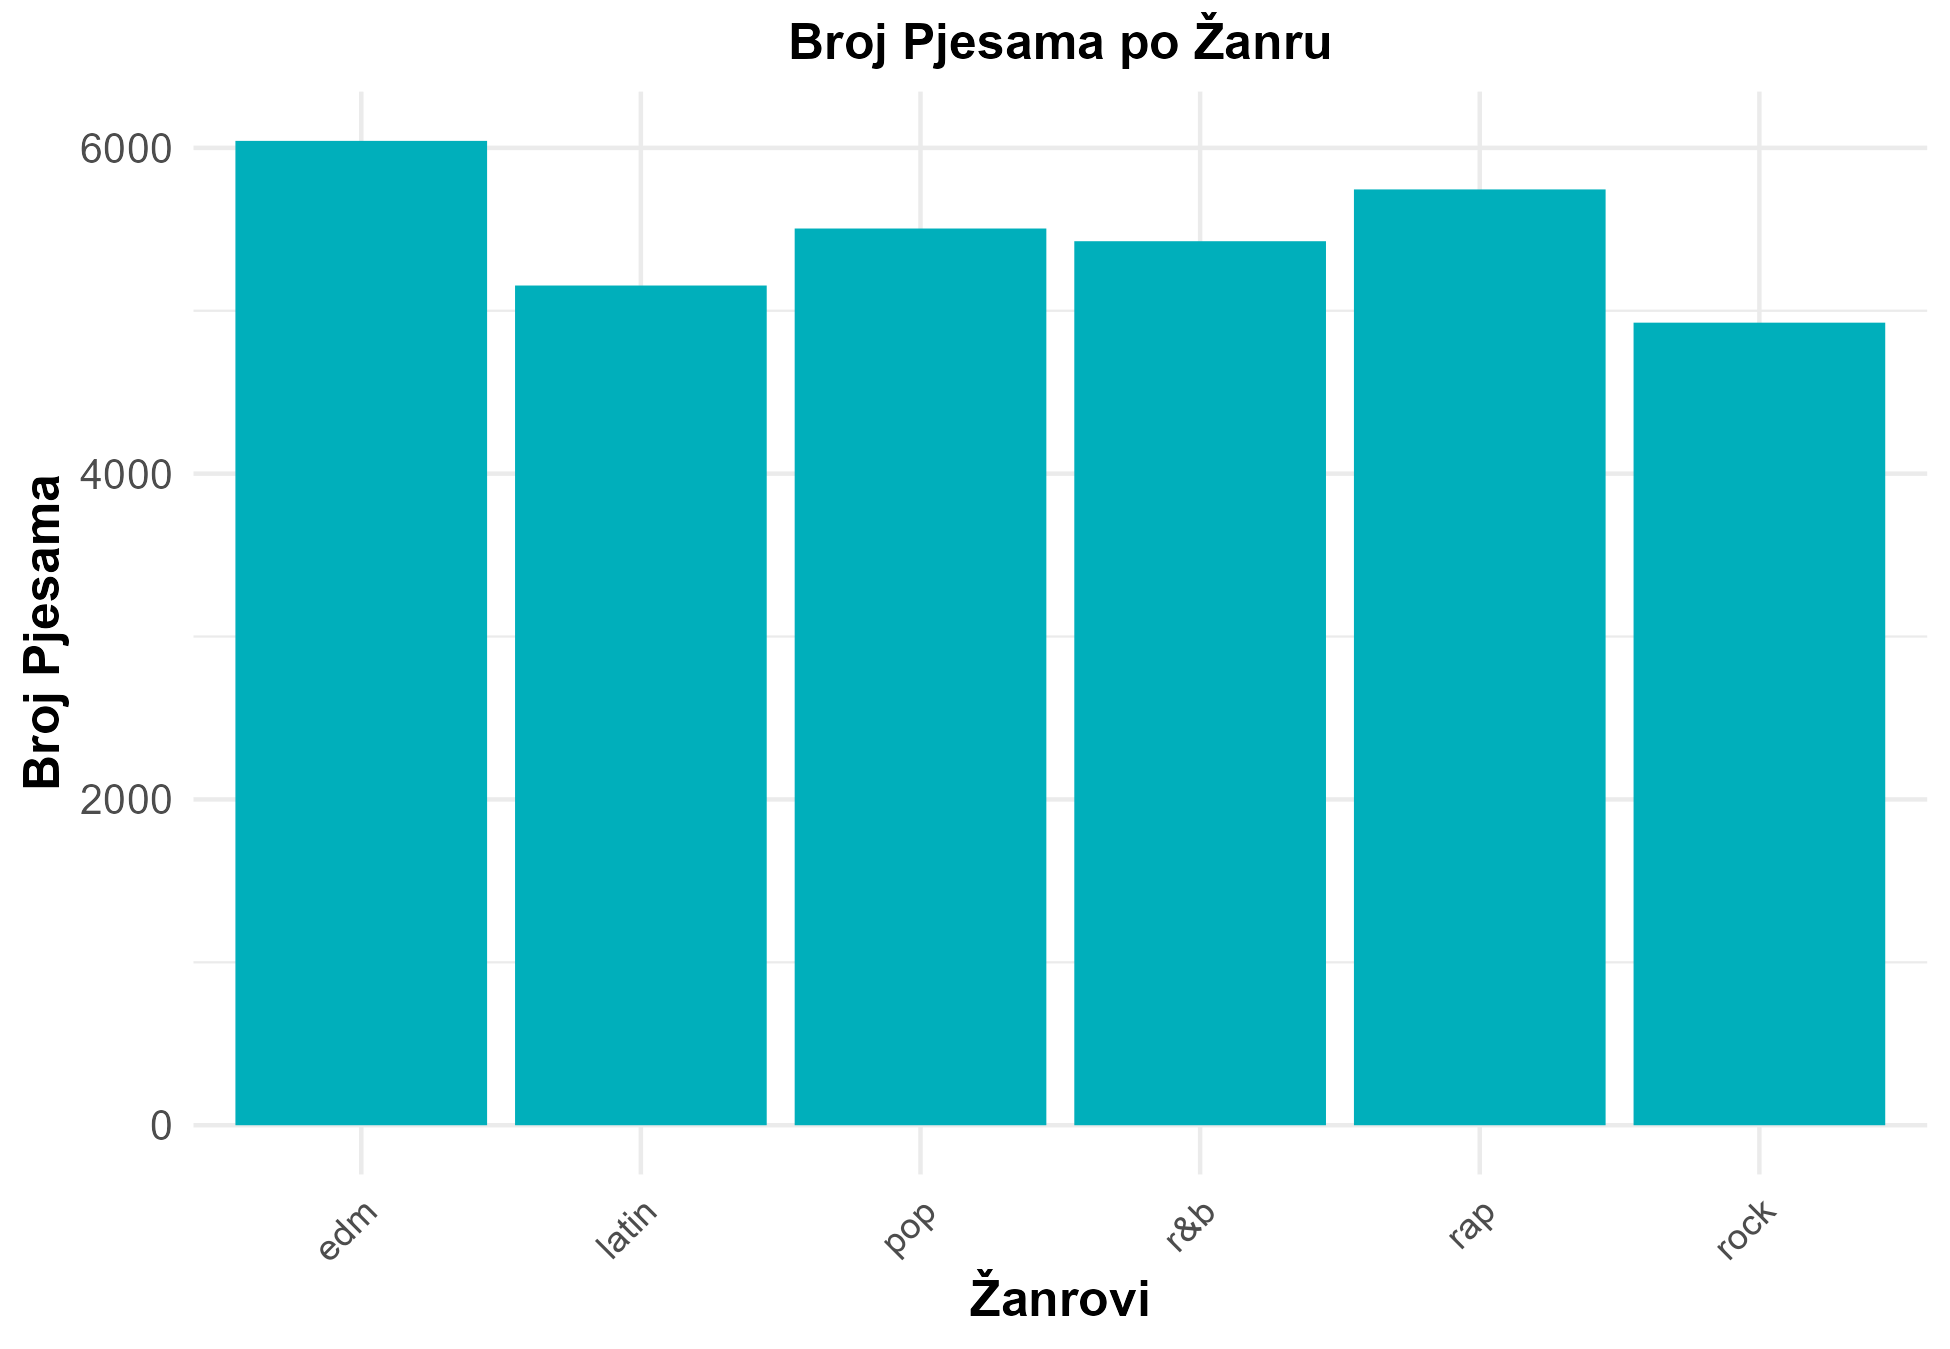
\includegraphics{popularnost_zanrova.png}

\textbf{Analiza grafa}

Graf ``Broj Pjesama po Žanru'' vizualno prikazuje raspodjelu glazbenih
žanrova Spotify datasetu. Svaki stupac na grafu predstavlja određeni
glazbeni žanr, dok visina stupca odražava broj pjesama u tom žanru.

Ovaj graf pruža početni uvid u glazbene preferencije i raznolikost
žanrova među pjesmama na Spotifyju. Dominantni žanrovi mogu ukazivati na
popularnost određenih glazbenih stilova među korisnicima platforme.

Budući da je najpopulanriji edm (Electro dance music), prikazat ćemo
njegovu popularnost kroz godine

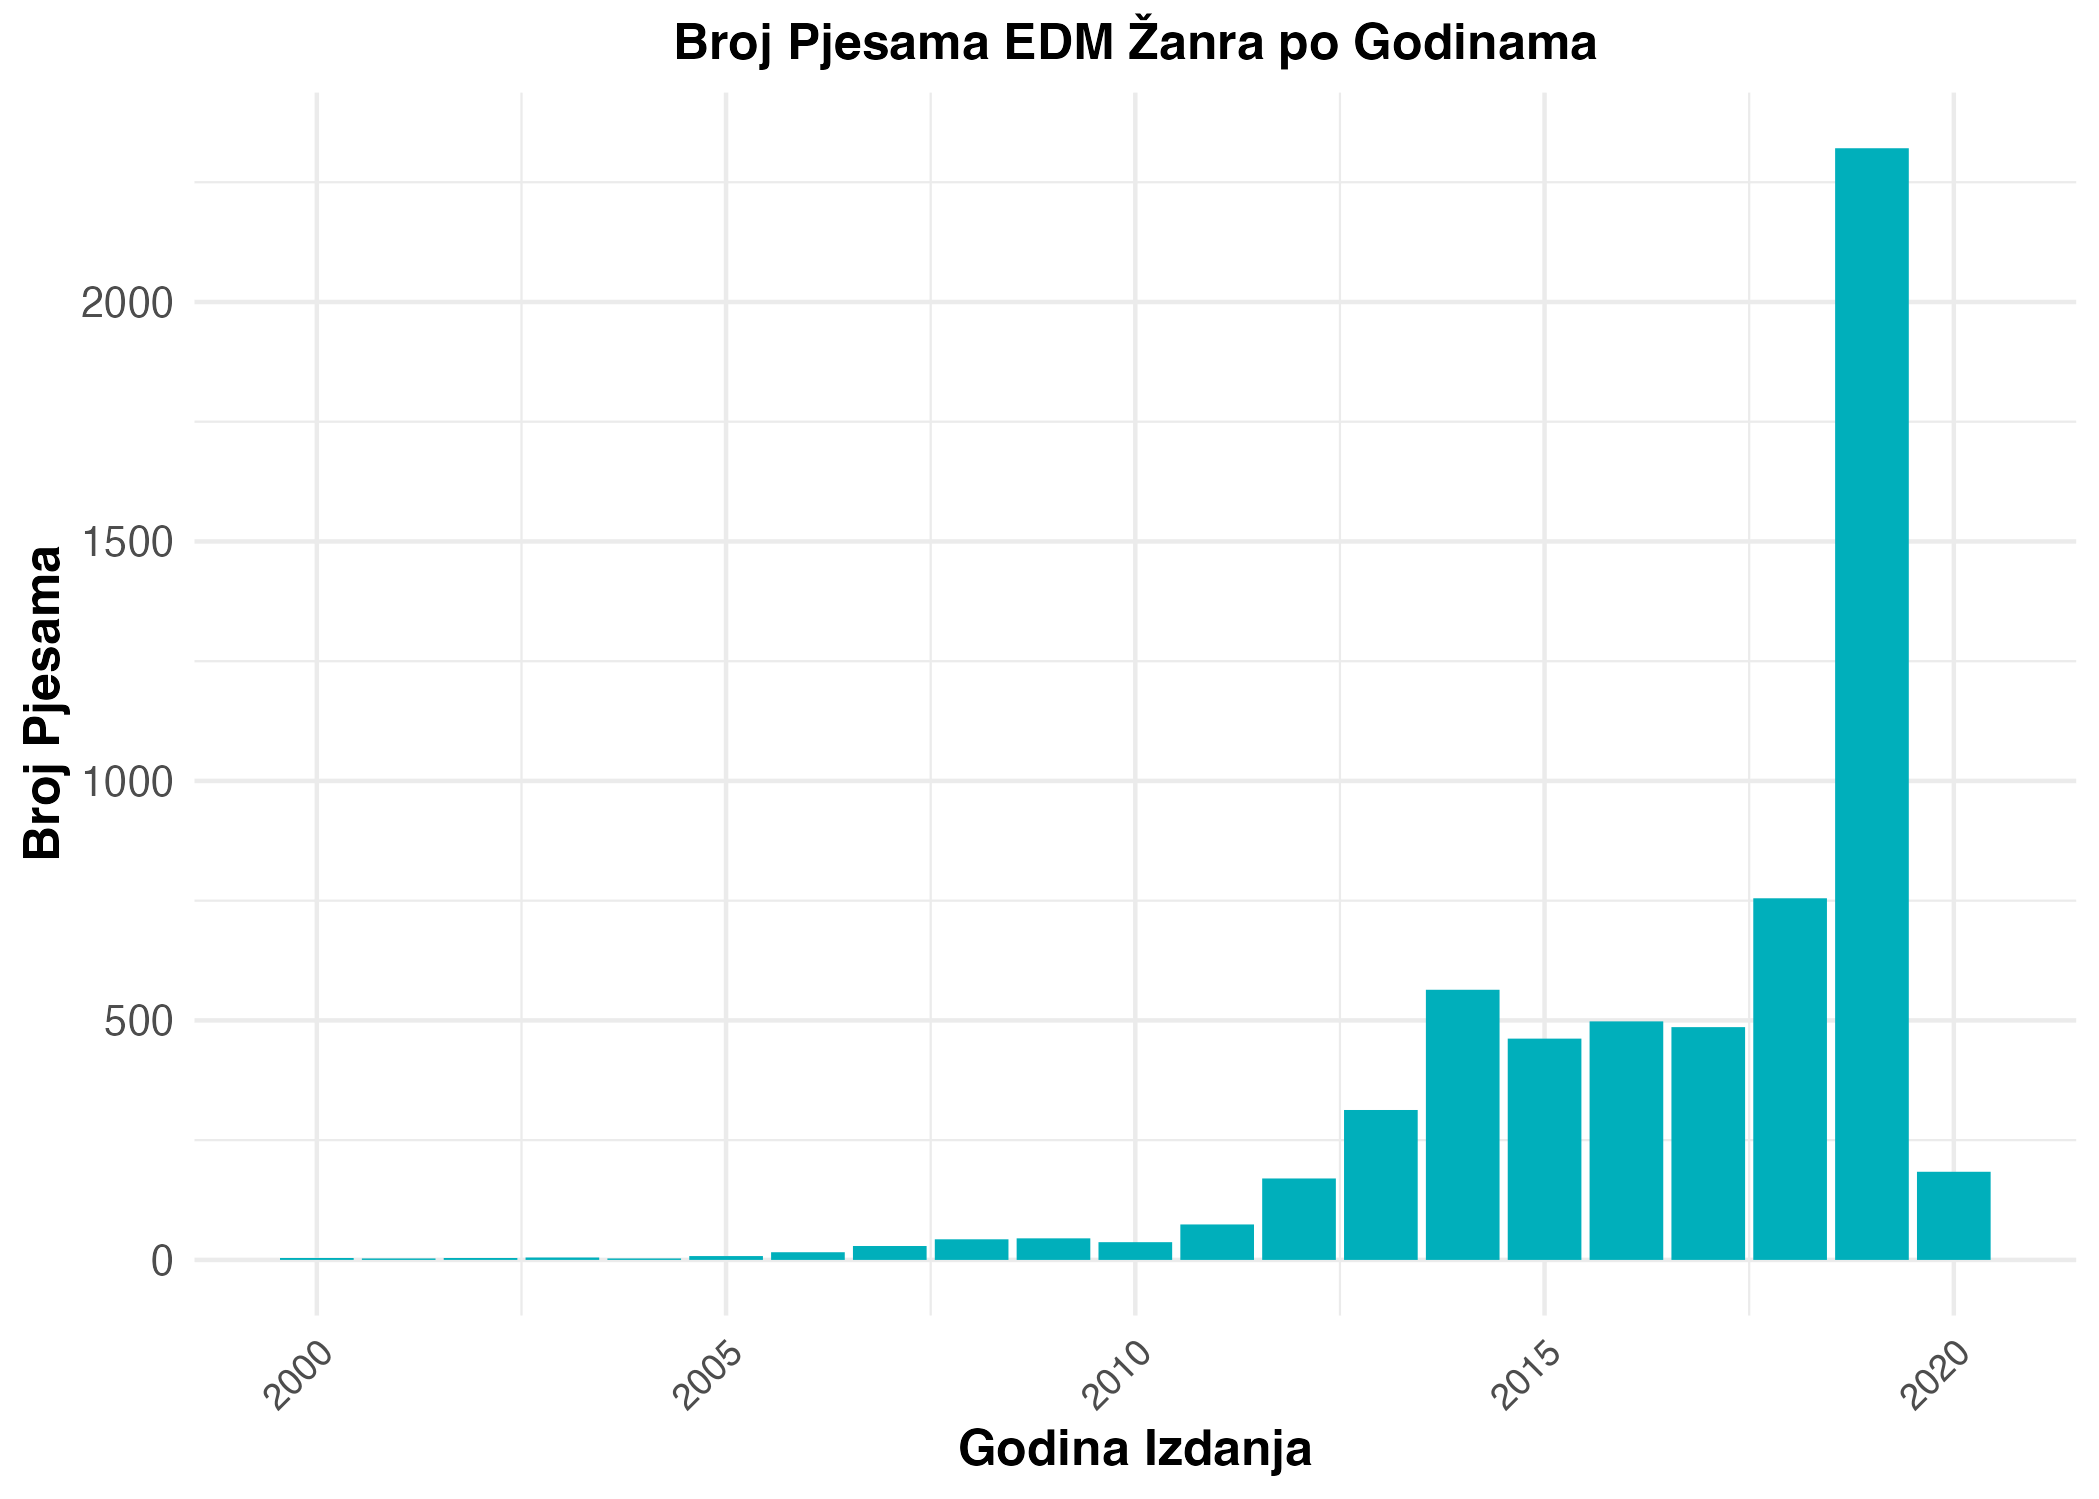
\includegraphics{broj_pjesama_EDM_zanra_po_god.png}

\textbf{Analiza grafa}

Graf ``Broj Pjesama EDM Žanra po Godinama'' vizualno prikazuje
raspodjelu glazbenog žanra EDM (Electro dance music) nad Spotify
datasetom. Svaki stupac na grafu predstavlja određenu godinu, dok visina
stupca odražava broj pjesama u toj godini.

Iz priloženog grafa može se zaključiti kako je edm (Electro dance music)
postao sve više popularan tek od 2012 godine, te od tada sve više
preuzima mainstream glazbe na Spotifyu.

\textbf{Najpopularniji izvodaci}

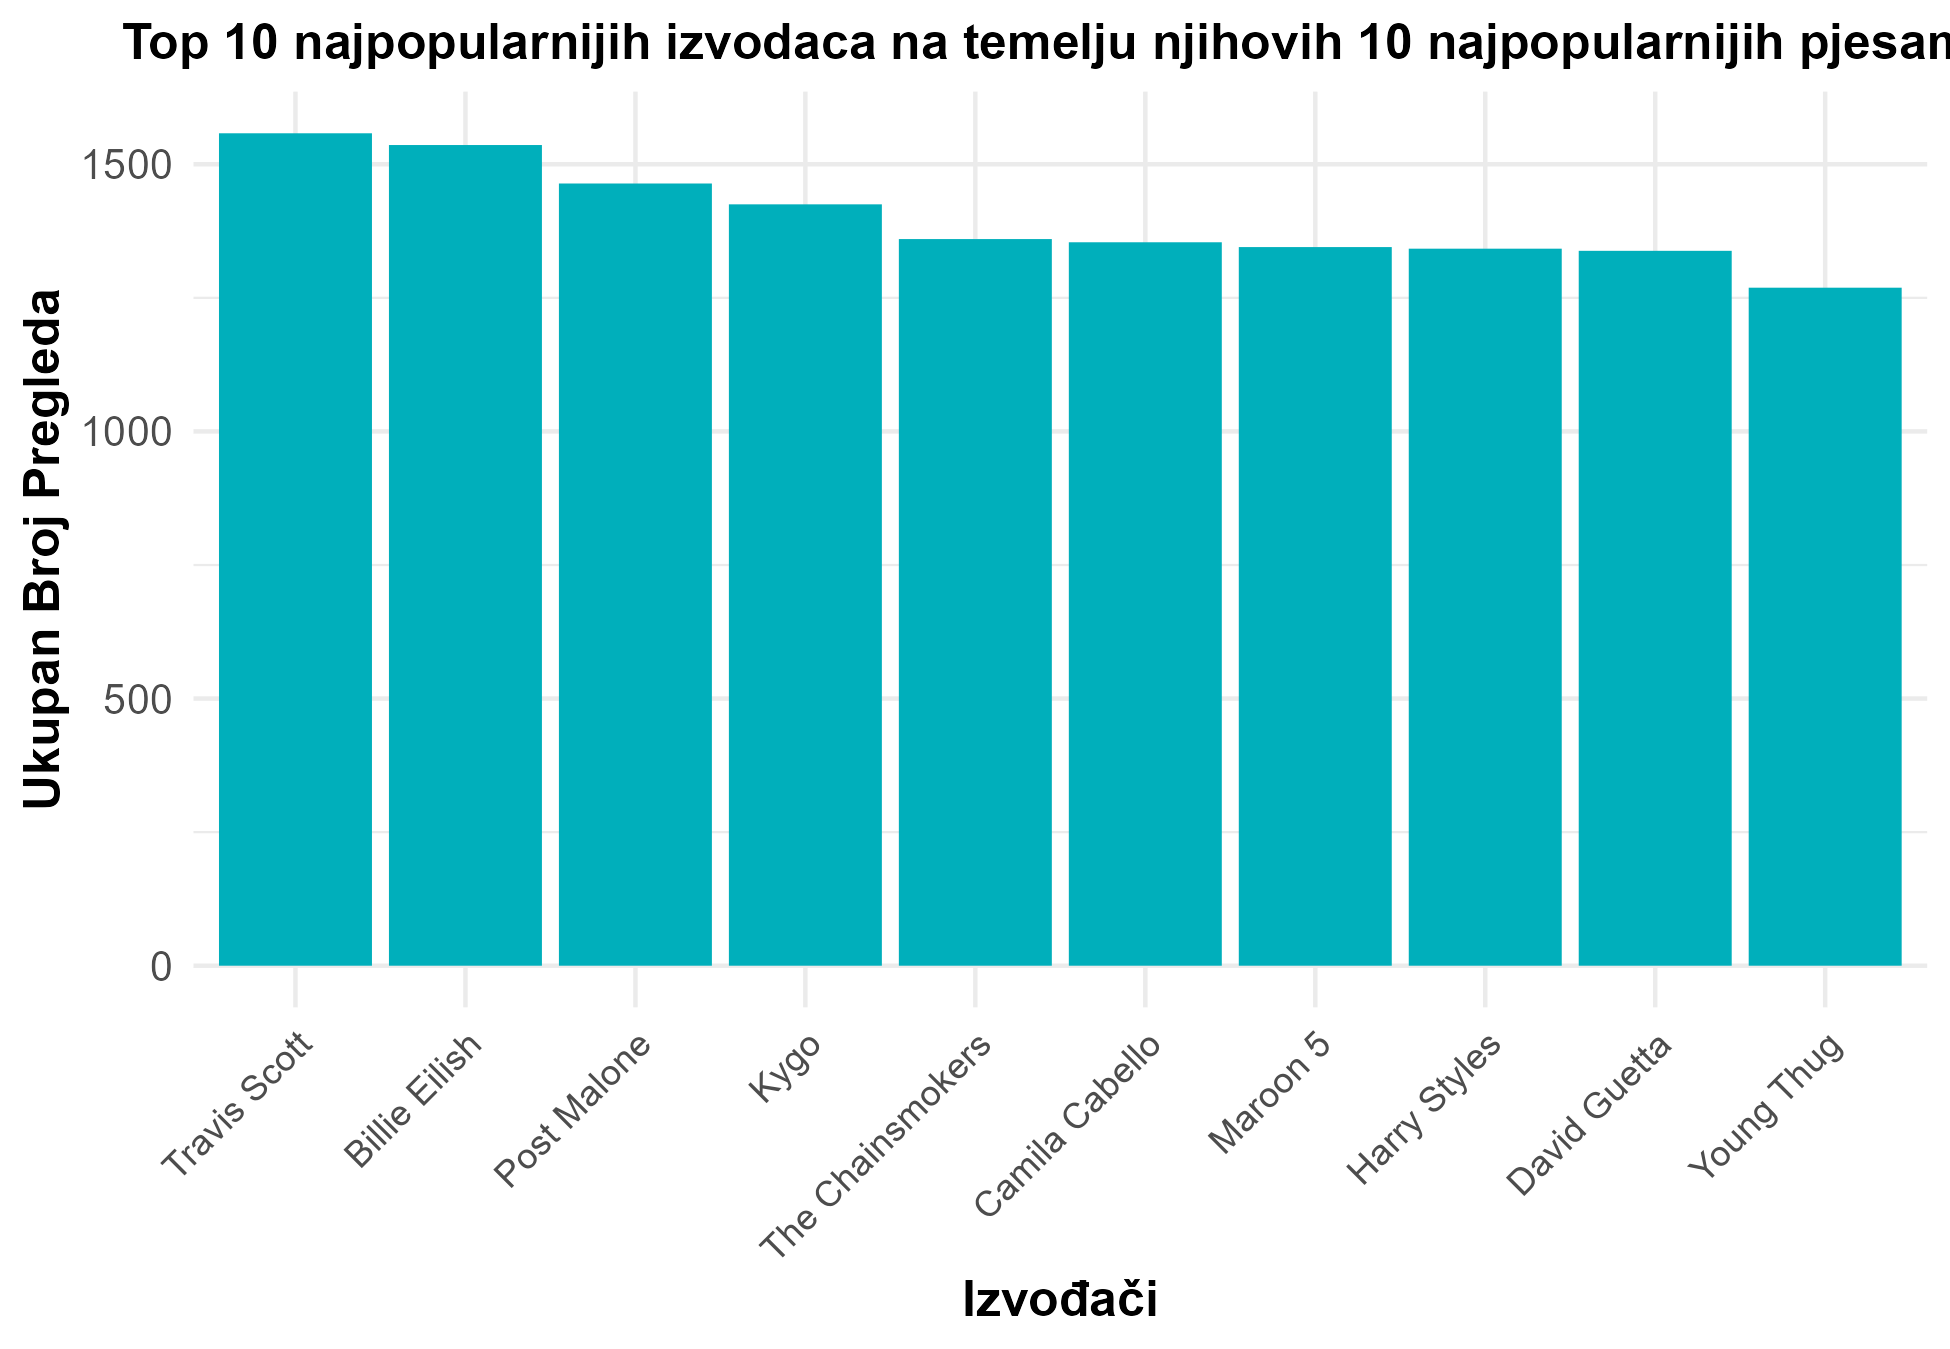
\includegraphics{najpopularniji_izvodaci.png} \textbf{Analiza grafa}

Grafički prikaz ukupnog broja pregleda temeljem 10 najpopularnijih
pjesama svakog izvođača pruža zanimljiv uvid u popularnost umjetnika na
Spotify platformi. Analizirajući graf, uočavamo da je Travis Scott
apsolutni lider među izvođačima, slijedi ga Billie Eilish, Post Malone
te ostali.

\textbf{Najpopularnije pjesme Travis Scotta}

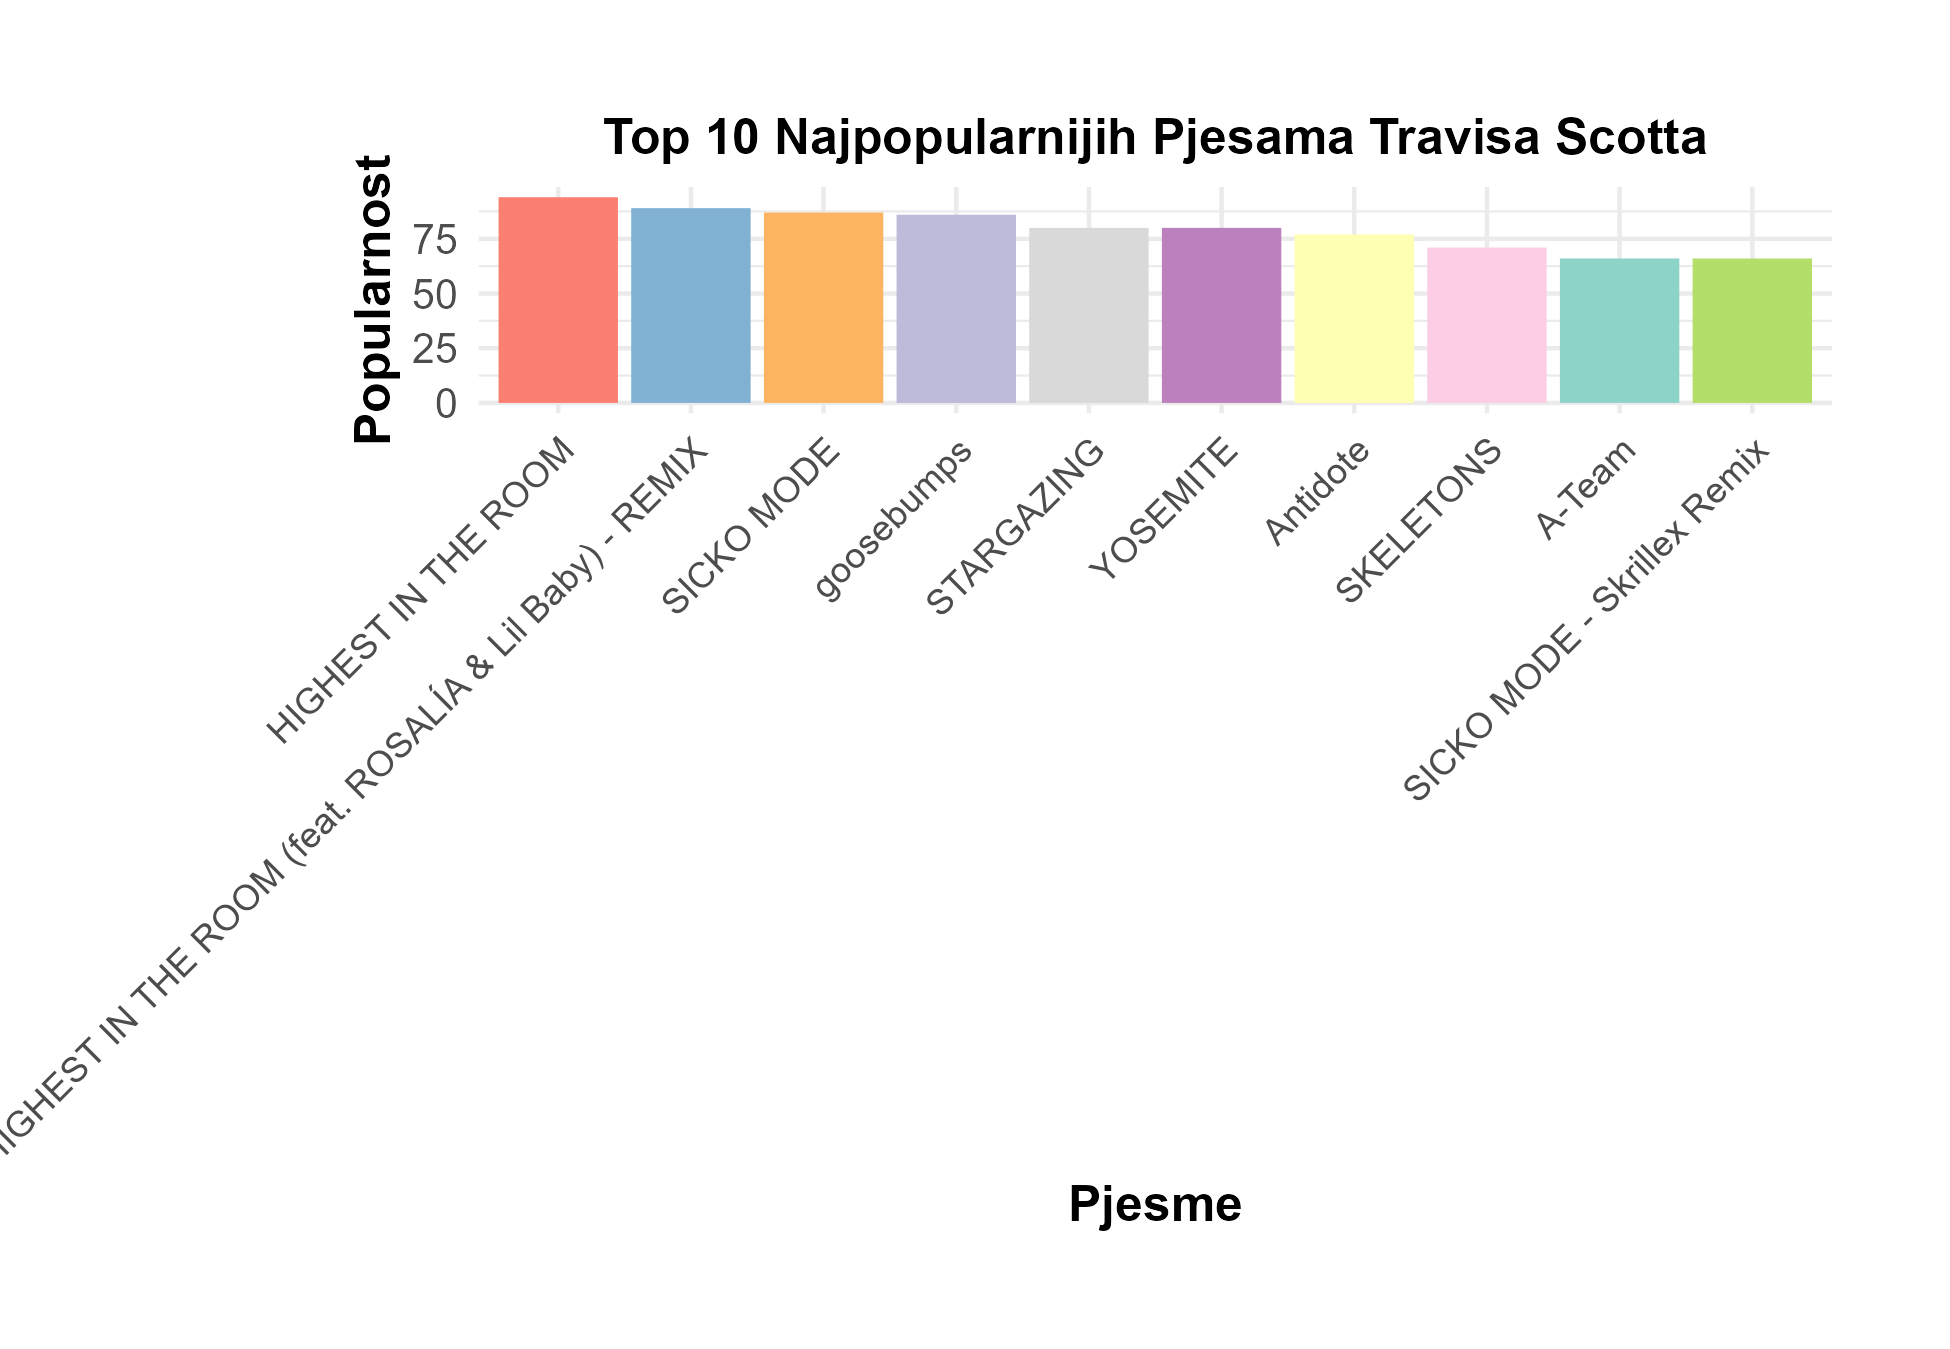
\includegraphics{travis_scott.png} \textbf{Analiza grafa}

Ova analiza naglašava impresivnu popularnost Travisa Scotta na Spotify
platformi, pri čemu se ističe njegov utjecaj kroz deset najpopularnijih
pjesama. ``Highest in the Room'' dominira među njima, zatim slijedi
istoimeni Remix, ``Sicko mode'' i ostali. Presudila je njegova
konstantnost jer nije samo bljesnuo s jednom pjesmom, već u svima drži
jako visoku kvalitetu izvedbe.

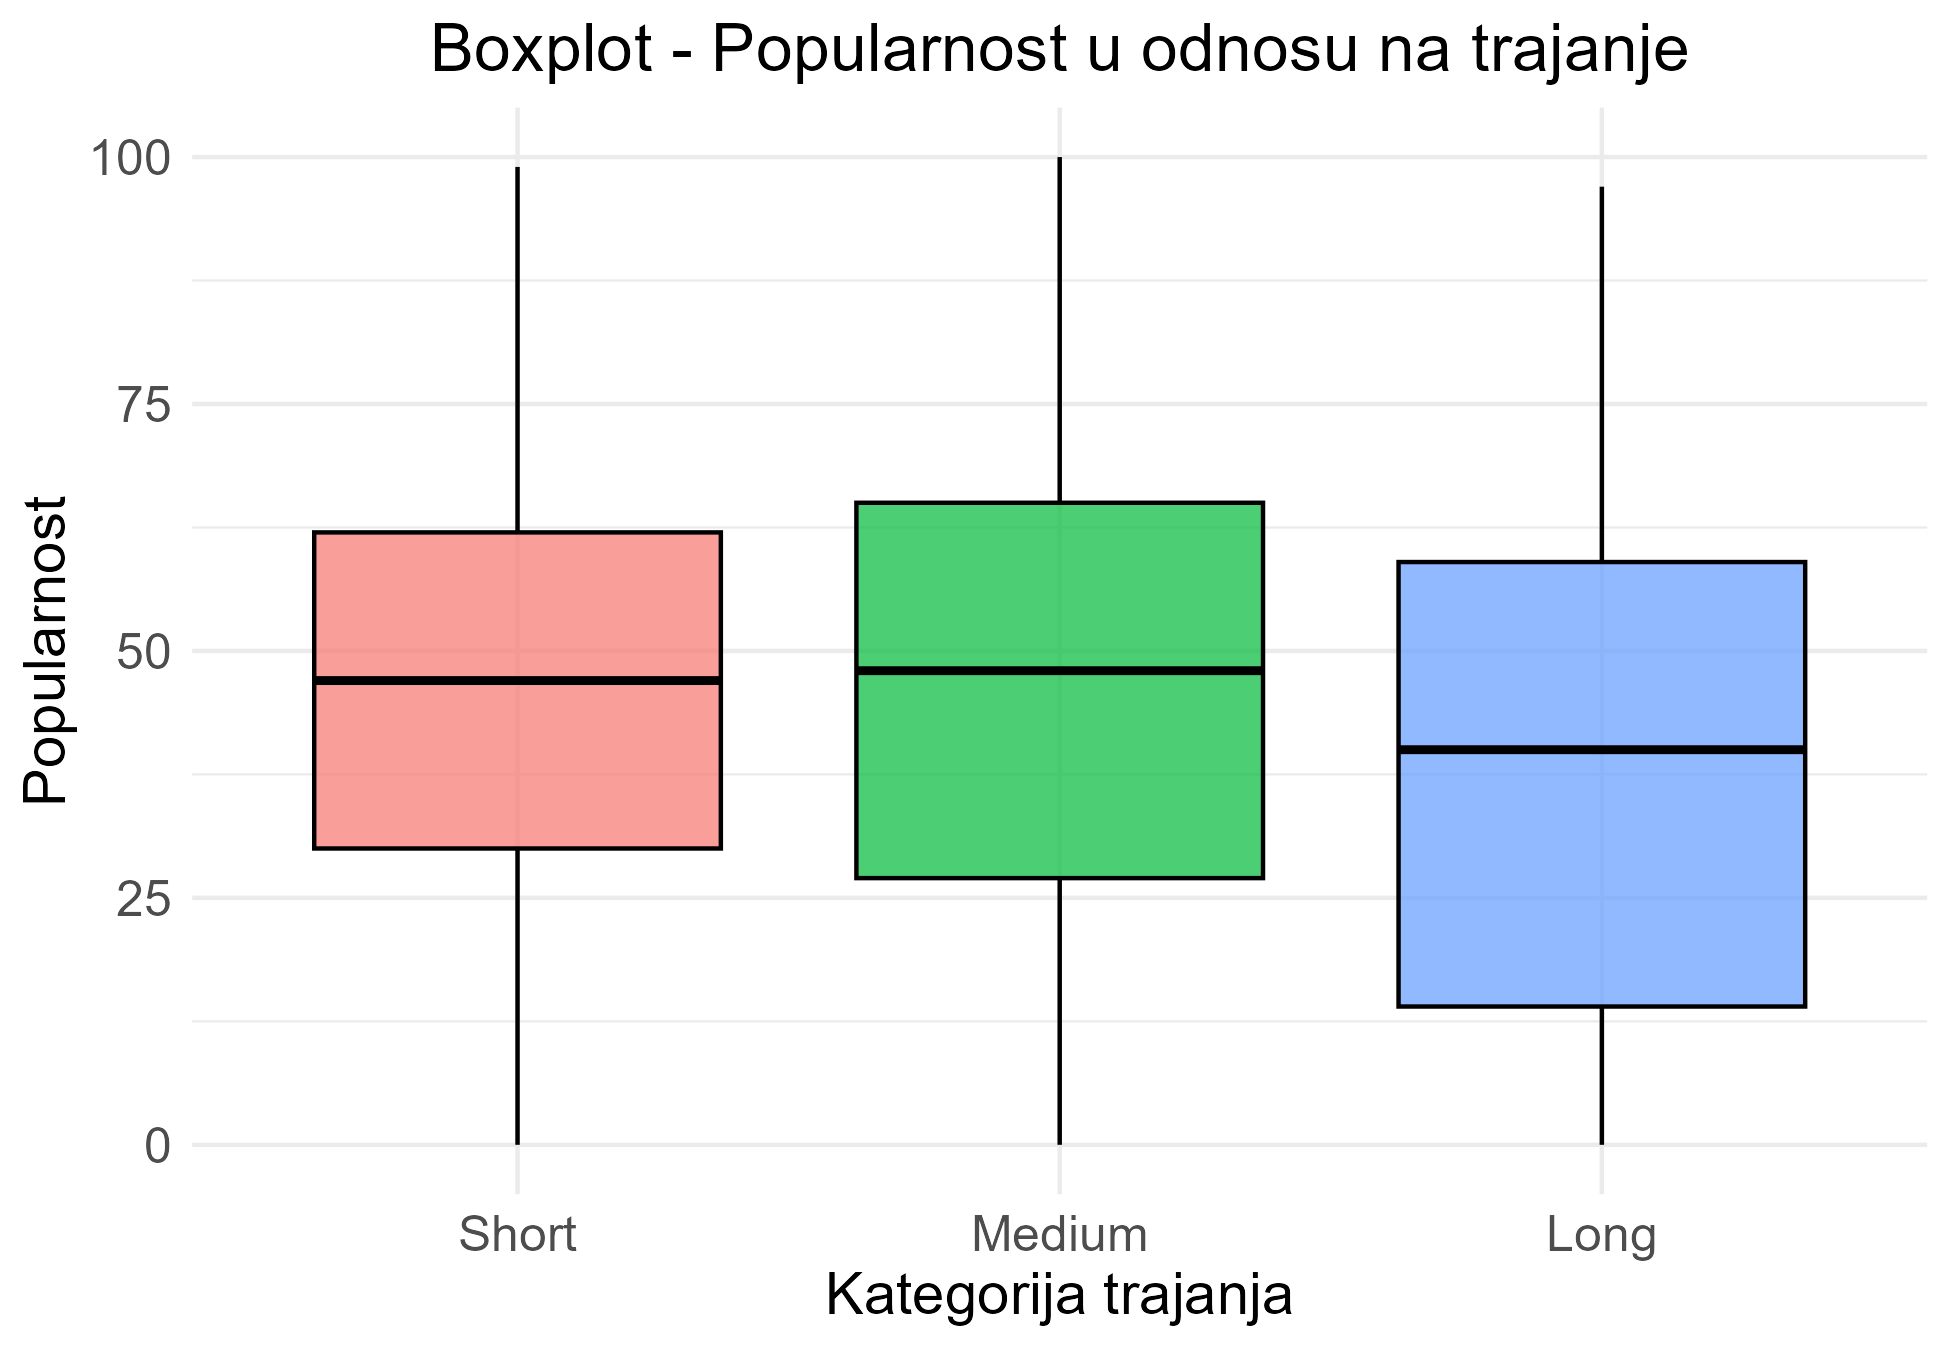
\includegraphics{graf1.png} 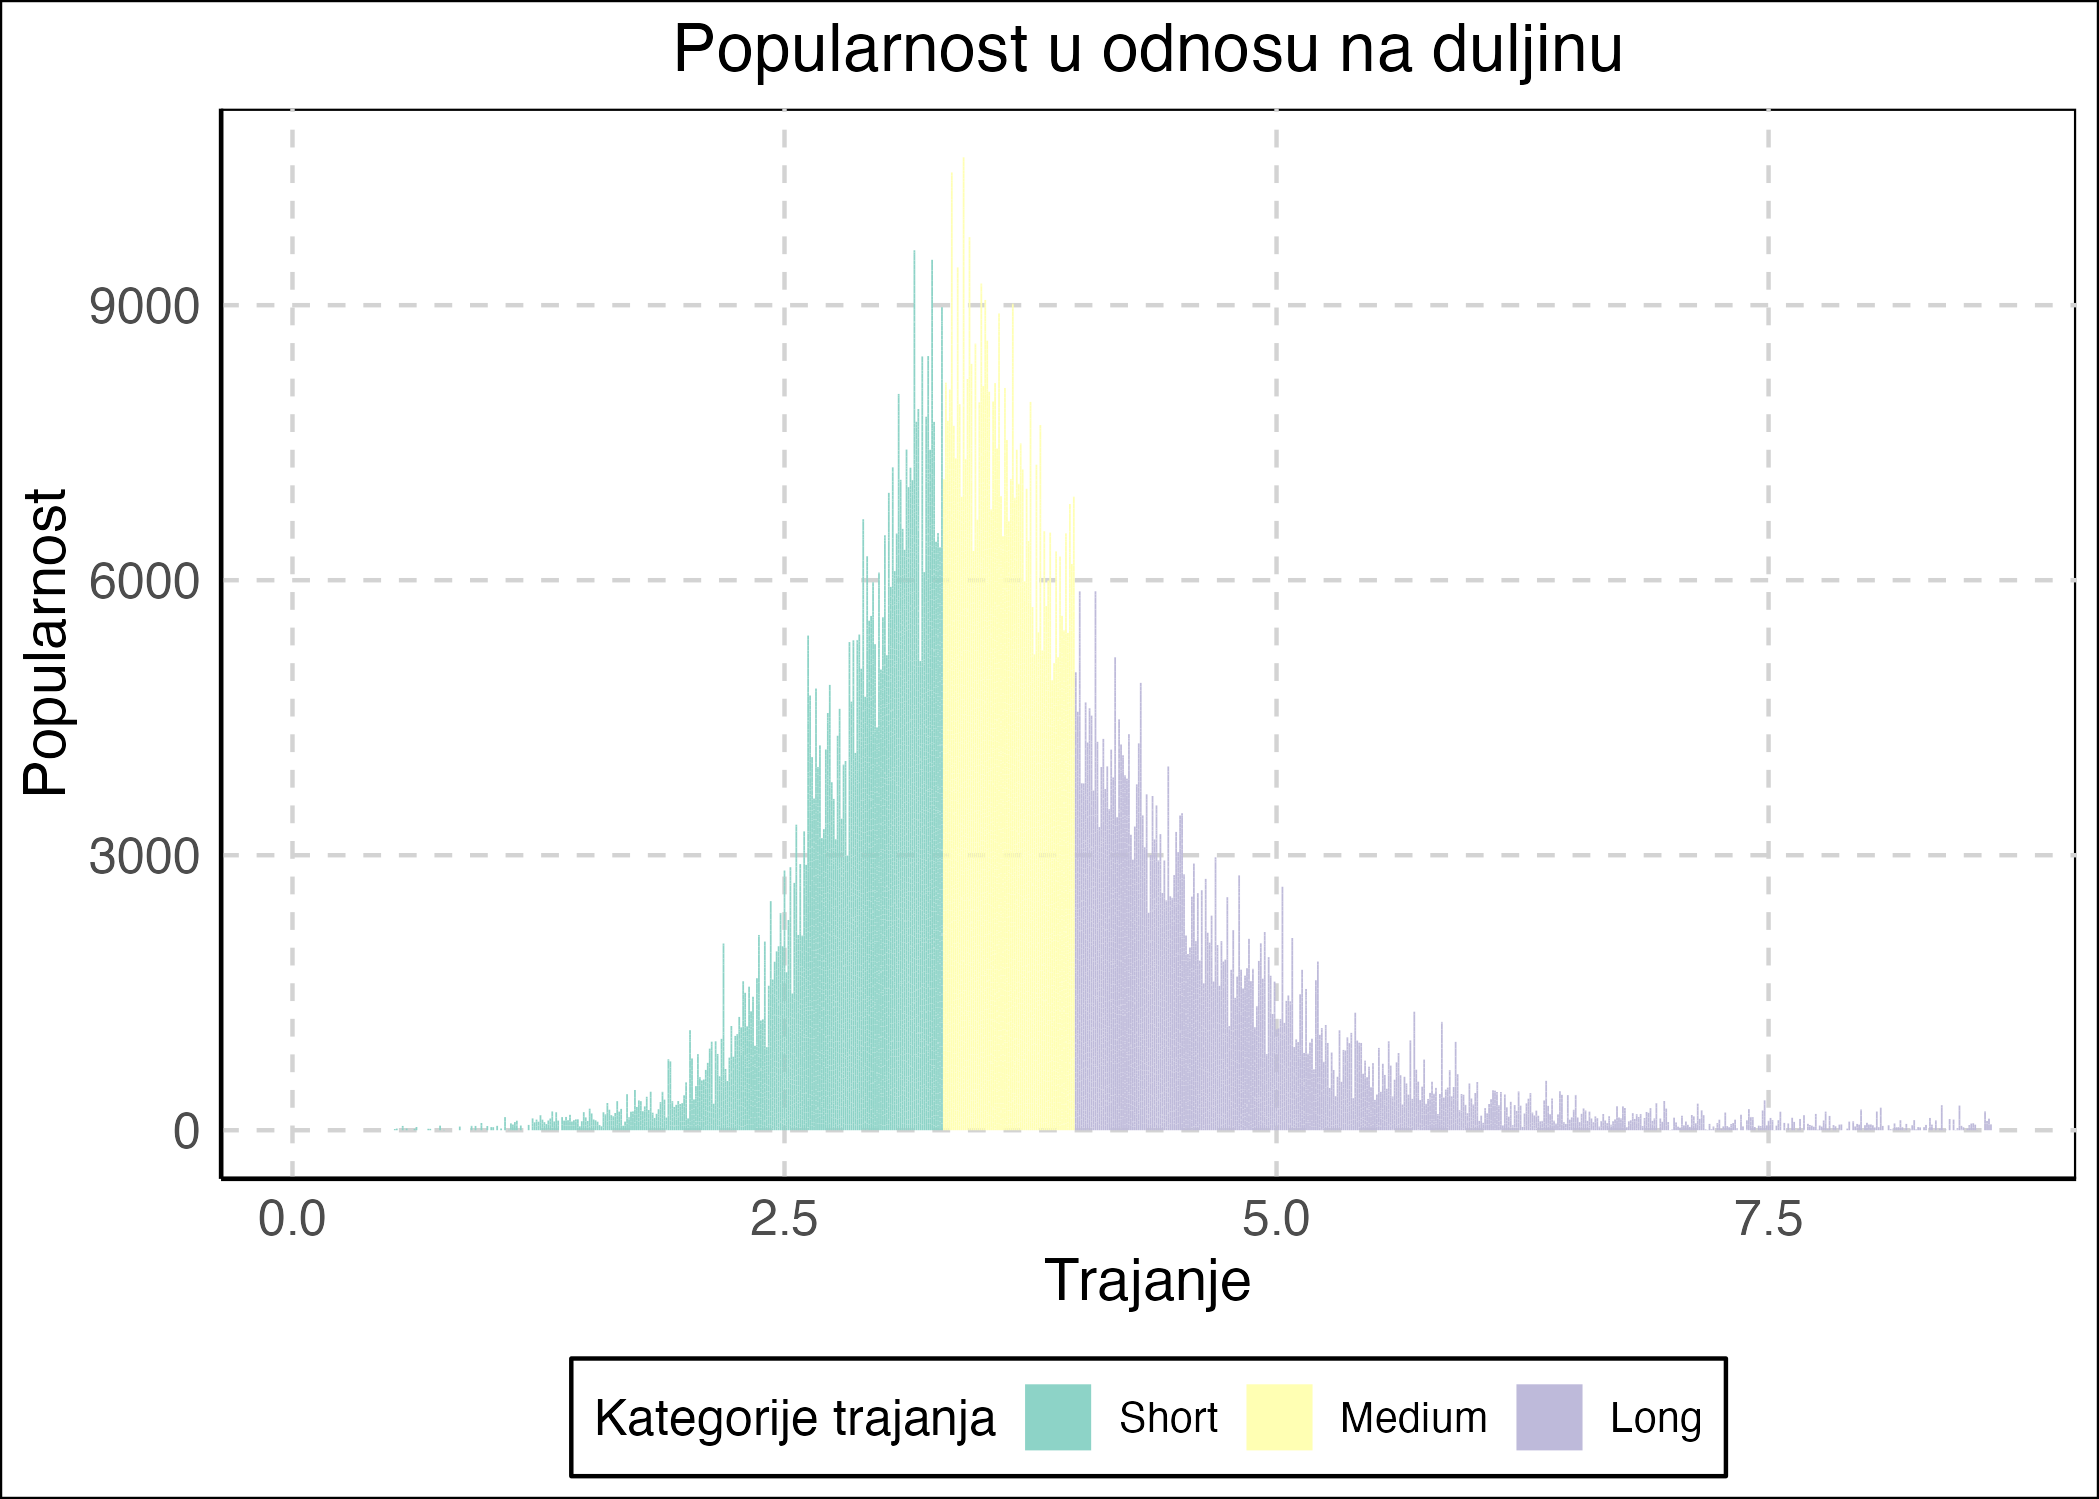
\includegraphics{graf2.png} \textbf{Analiza
grafa} Podijelili smo trajanje pjesama u 3 jednake kategorije, Short,
Medium, Long. Graf ``Boxplot - Popularnost u odnosu na trajanje''
prikazuje odnose Q1, Q2 i Q3 metrika koje se odnose na popularnost
pjesama pripadajuće kategorije. Iz priloženog se vidi da je medijan
popularnosti za duge pjesme znatno niži nego što možemo reći sa kratke i
srednje. Tu tvrdnju samo podupire graf ``Popularnost u odnosu na
duljinu'' koji prikazuje da su srednje pjesme najpopularnije, na drugom
mjestu su kratke, a daleko ispod njih se nalaze duge pjesme

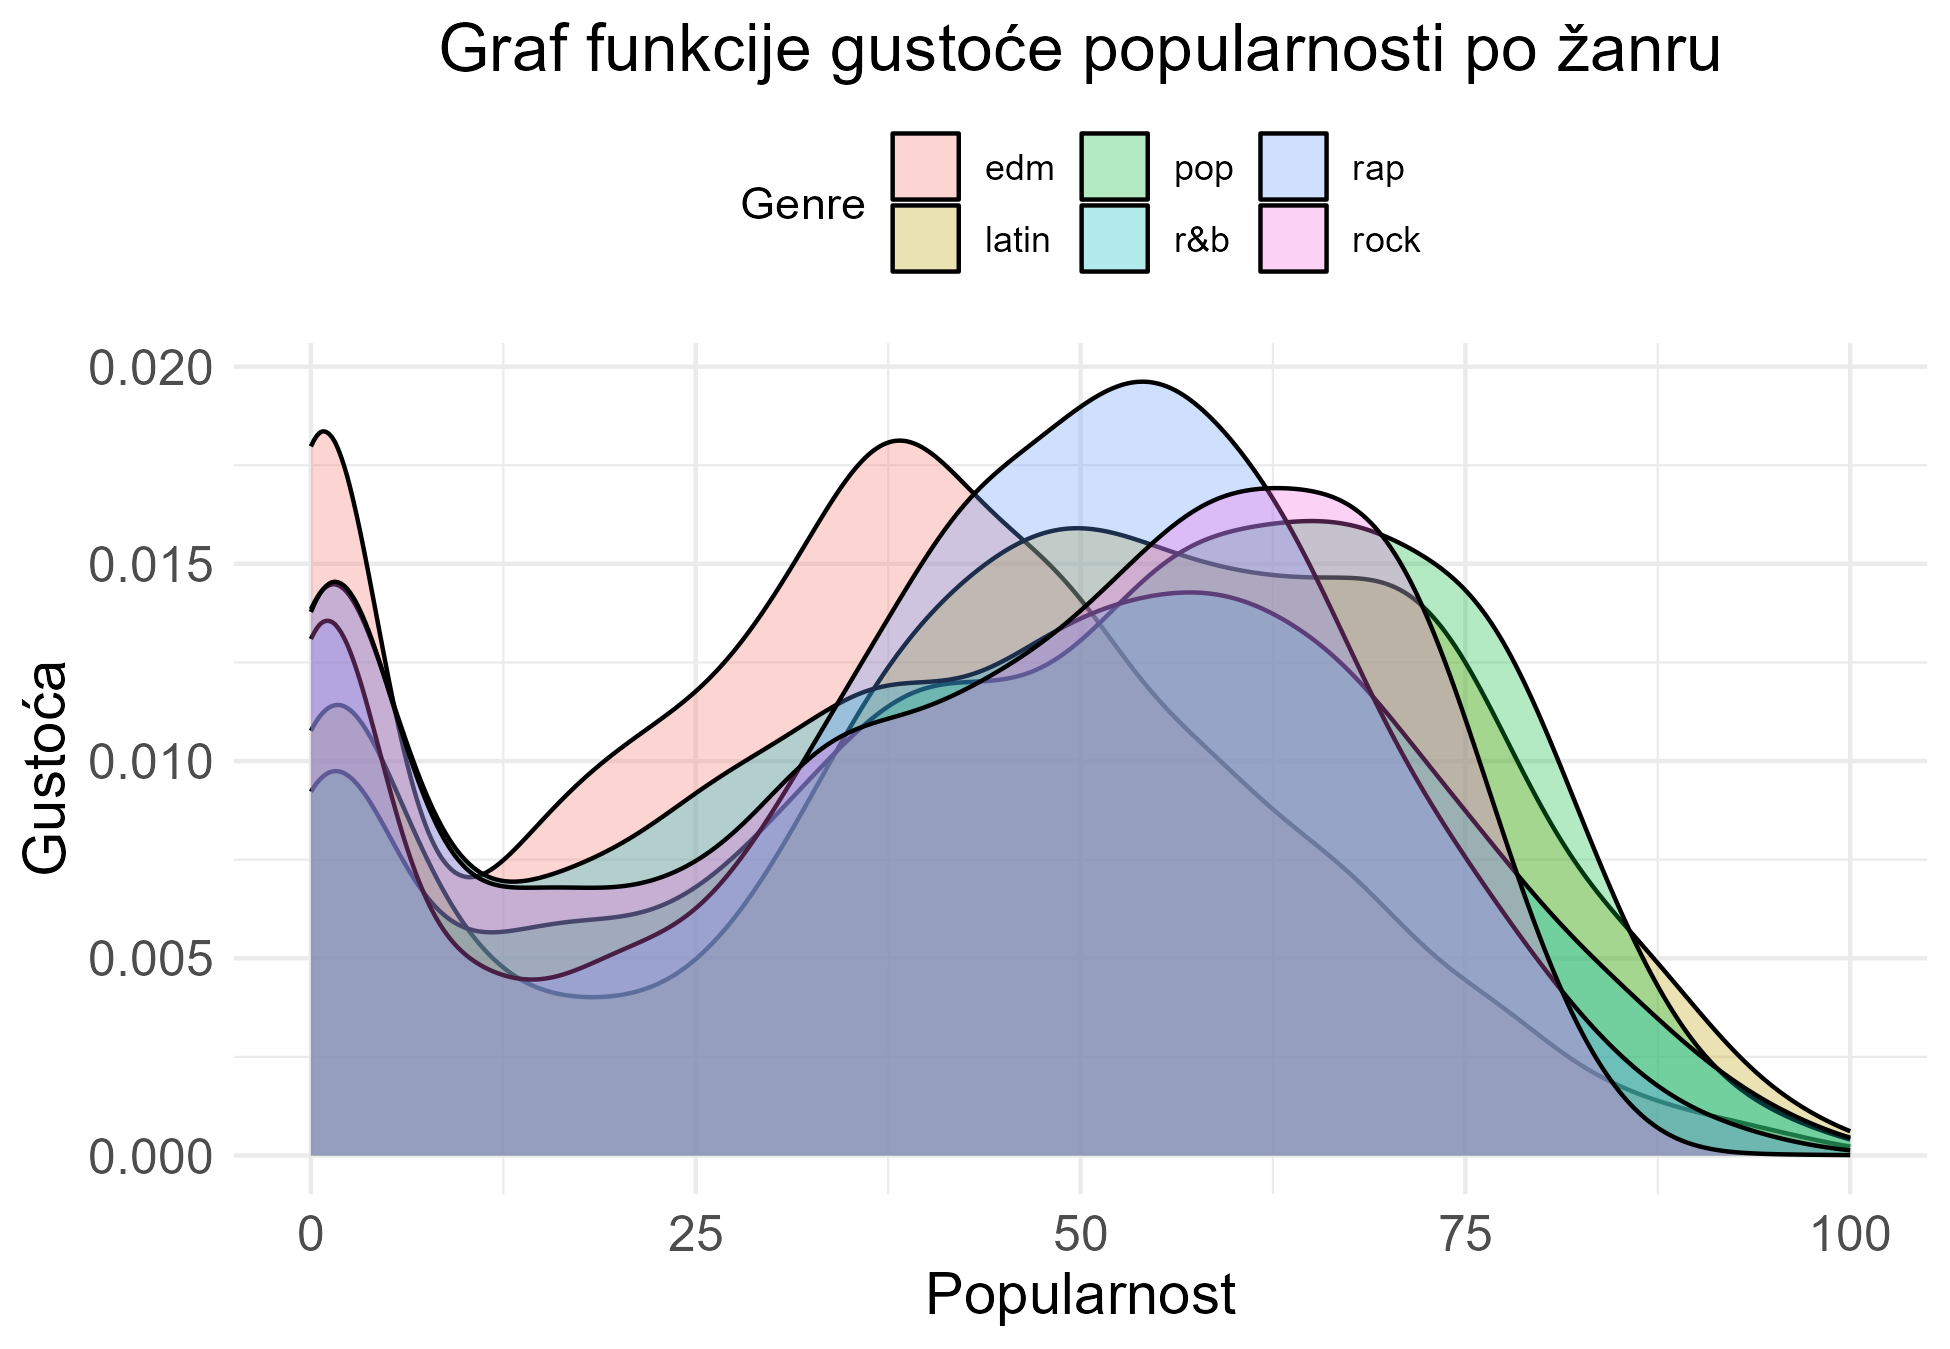
\includegraphics{graf3.png} \textbf{Analiza grafa} Iz grafa ``Graf
funkcije gustoće popularnosti po žanru'' možemo zaključiti da većinom
funkcije gustoća svih žanrova donekle prate normalnu razdiobu, stime da
sve imaju veliku devijaciju u lijevom repu. Naime Žanr ``edm'' ima
najviše malo popularnih pjesama, dok ``pop'' najmanje. Najviše srednje
ocjenjenih pjesama pripadaju žanru ``rap'', dok u najbolje ocjenjenim
pjesmama prednjači žanr ``latin''

\#\# ZAKLJUČAK \#\# Na samom početku smo napravili potrebne pretvorbe
podataka, i pretvorbe tipova podataka u one koje omogućavaju lakšu
analizu. Nakon toga nam je ostao podatknovni skup na kojem je puno laške
izvoditi analize koje nas zanimaju. Iz grafa ``Broj Pjesama po Žanru''
vidimo da svakom žanru pripadaju od okvirno 5000 do 6000 pjesama. Za
bližu analizu broja novih pjesama kroz godine smo uzeli žanr ``edm'' i
to smo predstavili u grafu ``Broj Pjesama EDM Žanra po Godinama''. Iz
grafa možemo isčitati da je žanr bio relativno nepopularan do 2015.
godine, a posebice do 2010. godine. Nakon 2015. godine žanr uživa puno
veću popularnost i dostiže brojke od čak više od 2000 novih pjesama
godišnje netom prije 2020. godine. Zatim smo obradili popularnost samih
izvođača i njihovih pjesama. Grafički prikaz ukupnog broja pregleda
temeljem 10 najpopularnijih pjesama svakog izvođača pruža intrigantan
uvid u popularnost umjetnika na Spotify platformi. Analizom grafa ističe
se da je Travis Scott apsolutni lider među izvođačima. Ova analiza
naglašava impresivnu popularnost Travisa Scotta na Spotify platformi,
ističući njegov utjecaj kroz deset najpopularnijih pjesama. Posebno se
ističe ``Highest in the Room'' kao dominantna pjesma. Ključna je
Travisova konstantnost, ne samo s jednom pjesmom, već s održavanjem
visoke kvalitete izvedbe u svim pjesmama.Nakon toga smo se odlučili
analizirati odnos popularnosti i trajanja pjesme tako što smo trajanje
podjelili u 3 podjednake kategorije.Iz grafova ``Boxplot - Popularnost u
odnosu na trajanje'' i ``Popularnost u odnosu na duljinu'' vidimo kako
su dulje pjesme u glavnom lošije ocjenjene u odnosu na pjesme koje su
kratke ili srendnje, koje prednjače u popularnosti. Za kraj odlučili smo
se na analizu funckije gustoće popularnosti pojedinih žanrova što smo
vizualizirali u grafu ``Graf funkcije gustoće popularnosti po žanru''.
Vidimo da po broju nisko ocjenjenih pjesama pobjedu odnosi žanr ``edm''
dok žanr ``rap'' prednjači po srednje ocjenjenim pjesmama, a u najboljim
pjesmama se ističe žanr ``latin''.

\end{document}
